No aplicativo de simulações do programa \emph{Matlab\tiny\textregistered}, \emph{Simulink}, cria-se no ambiente de simulações o seguinte diagrama de blocos:\\
\begin{figure}[H]
		\centering
		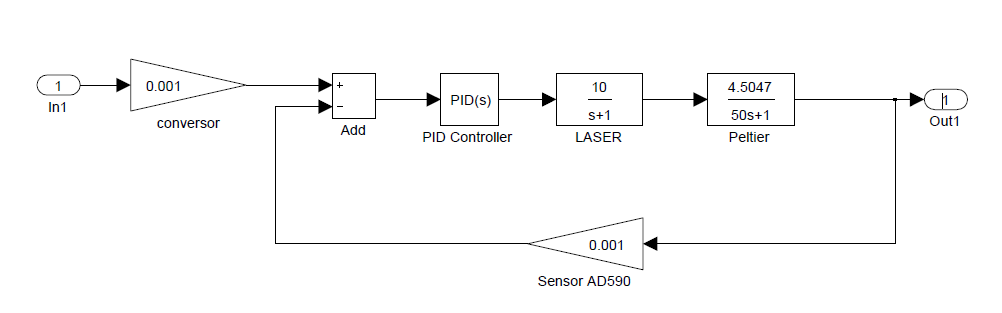
\includegraphics[width=0.8\linewidth]{./ima/PID-Final01.png}
		%\caption{}
		\label{fig:Ensaio1}
		\caption{Diagrama De Blocos emissor de LASER}
	\end{figure}
	
Em seguida executasse a simulação e análise do sistema onde obtemos os melhores parâmetros para os ganhos de Kp ( proporcional), Ki ( integral ) e Kd ( diferencial ) para os quais a resposta seja mais rápida e atinja o valor de setpoint.\\
Os valores obtidos que melhor operaram o PID no ambiente de simulação do \emph{Matlab\tiny\textregistered} Simulink foram os seguintes valores:\\
\textbf{$K_{p}= 390;  K_{d}= 11;  K_{i}= 20$} \\
\paragraph{}
Para estes valores, a resposta bem rápida e com o valor de set point parametrizado em Volts [V], podemos adotar uma larga faixa de ajustes de temperatura.\\
Seguem os dados obtidos da simulação:\\ 

\begin{figure}[H]
		\centering
		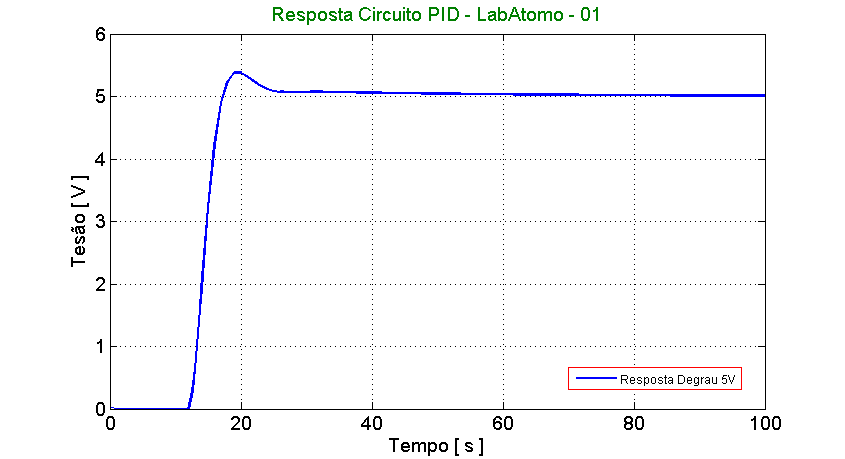
\includegraphics[width=0.7\linewidth]{./ima/LabAtomo01.png}
		%\caption{}
		\label{fig:simulinkA1}
		\caption{Curva de resposta ao degrau de 5V - Set point}
	\end{figure}
Com estes ajustes de ganho obtidos através da simulação, temos os seguintes valores para os resistores e capacitores do circuito, utilizando-se de valores comerciais temos:\\

%%% Tabela de dados do PID 

% Please add the following required packages to your document preamble:
% \usepackage[table,xcdraw]{xcolor}
% If you use beamer only pass "xcolor=table" option, i.e. \documentclass[xcolor=table]{beamer}
\begin{table}[H]
\centering
\caption{Parâmetros elementos de circuito PID}
\label{Paramentros PID}
\begin{tabular}{|l|l|l|}
\hline
\rowcolor[HTML]{FCFF2F} 
\multicolumn{1}{|c|}{\cellcolor[HTML]{FCFF2F}\textbf{Kp}} & \multicolumn{1}{c|}{\cellcolor[HTML]{FCFF2F}\textbf{Ki}} & \multicolumn{1}{c|}{\cellcolor[HTML]{FCFF2F}\textbf{Kd}} \\ \hline
$R_{1}= 1 K\Omega$                                       & $C_{2}= 47 \mu F$                                       & $C_{1}= 47\mu F$                                        \\ \hline
$R_{2}= 390 K\Omega$                                     & $R_{5}= 1069 \Omega$                                    & $R_{4}= 75 k\Omega$                                     \\ \hline
$R_{2 comercial} = 220 K\Omega$                          & $R_{5}= 700 \Omega$                                     & $R_{4}=60 K\Omega$                                      \\ \hline
$Trimpot = 1 volta 200 K\Omega$                             & $Trimpot = 1 volta 1 K\Omega$                              &$ Trimpot = 1 volta 10 K\Omega$                             \\ \hline
\end{tabular}
\end{table}

